\begin{activity} \label{A:3.5.2}  A television camera is positioned 4000 feet from the base of a rocket launching pad.  The angle of elevation of the camera has to change at the correct rate in order to keep the rocket in sight.  In addition, the auto-focus of the camera has to take into account the increasing distance between the camera and the rocket.  We assume that the rocket rises vertically.  (A similar problem is discussed and pictured dynamically at \href{http://gvsu.edu/s/9t}{\texttt{http://gvsu.edu/s/9t}}.  Exploring the applet at the link will be helpful to you in answering the questions that follow.)
\ba
	\item Draw a figure that summarizes the given situation.  What parts of the picture are changing?  What parts are constant?  Introduce appropriate variables to represent the quantities that are changing.
	\item Find an equation that relates the camera's angle of elevation to the height of the rocket, and then find an equation that relates the instantaneous rate of change of the camera's elevation angle to the instantaneous rate of change of the rocket's height (where all rates of change are with respect to time).
	\item Find an equation that relates the distance from the camera to the rocket to the rocket's height, as well as an equation that relates the instantaneous rate of change of distance from the camera to the rocket to the instantaneous rate of change of the rocket's height (where all rates of change are with respect to time).
	\item Suppose that the rocket's speed is 600 ft/sec at the instant it has risen 3000 feet.  How fast is the distance from the television camera to the rocket changing at that moment?  If the camera is following the rocket, how fast is the camera's angle of elevation changing at that same moment?
	\item If from an elevation of 3000 feet onward the rocket continues to rise at 600 feet/sec, will the rate of change of distance with respect to time be greater when the elevation is 4000 feet than it was at 3000 feet, or less?  Why?  
\ea
\end{activity}
\begin{smallhint}
\ba
	\item Let $\theta$ represent the camera angle and note that one leg of the right triangle is constant.  Which two are changing?
	\item Think trigonometrically.
	\item Think like Pythagoras.
	\item Use the facts that $h = 3000$ and $\frac{dh}{dt} = 600$ in your preceding work.
	\item You can answer this question intuitively or by changing the value of $h$ in your work in (d).
\ea
\end{smallhint}
\begin{bighint}
\ba
	\item Let $\theta$ represent the camera angle and note that one leg of the right triangle is constant.  Note that both the hypotenuse and the vertical leg of the triangle are changing as the rocket rises.
	\item Think trigonometrically; which trigonometric function will only use the rocket's height along with the constant value of 4000?
	\item Use the Pythagorean Theorem to relate the three sides of the right triangle.
	\item Use the facts that $h = 3000$ and $\frac{dh}{dt} = 600$ in your preceding work.  Note that these only apply after you have completed the work of differentiation, because $h$ is changing, not constant at 3000 feet.
	\item You can answer this question intuitively or by changing the value of $h$ in your work in (d).
\ea
\end{bighint}
\begin{activitySolution}
\ba
	\item Letting $\theta$ be the camera's elevation angle, $h$ the rocket's height, and $z$ the distance from the camera to the rocket, we have the following situation at a given point in time:
	\begin{center}
	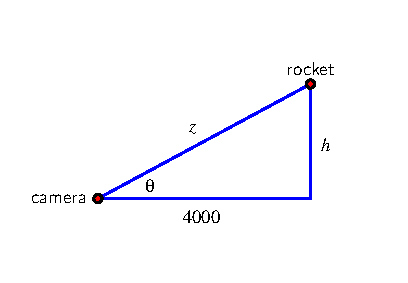
\includegraphics{figures/3_5_Act2Soln.eps}
	\end{center}
	\item To relate $\theta$ and $h$, observe that the tangent function is a good choice, since $\tan(\theta) = \frac{h}{4000}$, so that
	$$h = 4000 \tan(\theta).$$
	Differentiating implicitly with respect to $t$, we find that
	$$\frac{dh}{dt} = 4000 \sec^2 (\theta) \frac{d\theta}{dt}.$$
	\item To relate $z$ and $h$, the Pythagorean Theorem is natural to consider.  By this famous result, 
	$$h^2 + 4000^2 = z^2.$$
	Differentiating both sides implicitly with respect to $t$, it follows
	$$2h \frac{dh}{dt} = 2z \frac{dz}{dt},$$
	and thus $h \frac{dh}{dt} = z \frac{dz}{dt}.$
	\item Using the given fact that the rocket's speed is 600 ft/sec at the instant it has risen 3000 feet, we know that $\left. \frac{dh}{dt} \right|_{h=3000} = 600$.  Note further in the triangle that when $h = 3000$, it follows $z = 5000$, since the base leg of the triangle is constant at 4000, by using the Pythagorean Theorem.  Substituting this information from the instant $h = 3000$ into the equation that relates the rates of change of $z$ and $h$ found in (c), we find that 
	$$2 \cdot 3000 \cdot 600 = 2 \cdot 5000 \cdot \left. \frac{dz}{dt} \right|_{h=3000}.$$
	Solving for $\left. \frac{dz}{dt} \right|_{h=3000}$ we have 
	$$\left. \frac{dz}{dt} \right|_{h=3000} = \frac{1800}{5} = 360 \ \mbox{feet/sec}.$$
	
	To answer the question about how fast the camera angle is changing, we use the same information but now in the equation we found in (b) that relates the rates of change of $\theta$ and $h$:
	$$\frac{dh}{dt} = 4000 \sec^2 (\theta) \frac{d\theta}{dt}.$$
	Observe that when $h = 3000$, in the 3000-4000-5000 right triangle, it follows that $\cos(\theta) = \frac{4}{5}$, so $\sec(\theta) = \frac{5}{4}$.  Thus, using the instantaneous information,
	$$600 = 4000 \cdot \frac{25}{16} \left. \frac{d\theta}{dt} \right|_{h=3000},$$
	and thus
	$$ \left. \frac{d\theta}{dt} \right|_{h=3000} = \frac{6 \cdot 16}{40 \cdot 25} = \frac{12}{125},$$
	which is measured in radians per second.
	\item Recalling that $2h \frac{dh}{dt} = 2z \frac{dz}{dt}$, it follows that 
	$$\frac{dz}{dt} = \frac{h}{z} \frac{dh}{dt}.$$
	Using this equation when $h = 3000$ and $\frac{dh}{dt} = 600$ led us to conclude that $\left. \frac{dz}{dt} \right|_{h=3000} = \frac{3}{5} \cdot 600 = 360 \ \mbox{feet/sec}$.  If we instead use $h = 4000$, it follows that $z = 4000\sqrt{2}$, so that
	$$\left. \frac{dz}{dt} \right|_{h=4000} = \frac{4}{4\sqrt{2}} \cdot 600 \approx 424.26 \ \mbox{feet/sec}.$$
	Indeed, $\frac{dz}{dt}$ is an increasing function of $h$, provided that $\frac{dh}{dt}$ is constant, because we can write $h^2 + 4000^2 = z^2$, so $z = \sqrt{h^2 + 4000^2}$, making
	$$\frac{dz}{dt} = \frac{h}{\sqrt{h^2 + 4000^2}} \frac{dh}{dt} = \frac{h}{\sqrt{h^2 + 4000^2}} 600.$$
	It is straightforward to verify that $\frac{h}{\sqrt{h^2 + 4000^2}}$ is an increasing function of $h$.
\ea
\end{activitySolution}
\aftera





